\documentclass[12pt,letterpaper]{article}
\usepackage{graphicx,textcomp}
\usepackage{natbib}
\usepackage{setspace}
\usepackage{fullpage}
\usepackage{color}
\usepackage[reqno]{amsmath}
\usepackage{amsthm}
\usepackage{fancyvrb}
\usepackage{amssymb,enumerate}
\usepackage[all]{xy}
\usepackage{endnotes}
\usepackage{lscape}
\newtheorem{com}{Comment}
\usepackage{float}
\usepackage{hyperref}
\newtheorem{lem} {Lemma}
\newtheorem{prop}{Proposition}
\newtheorem{thm}{Theorem}
\newtheorem{defn}{Definition}
\newtheorem{cor}{Corollary}
\newtheorem{obs}{Observation}
\usepackage[compact]{titlesec}
\usepackage{dcolumn}
\usepackage{tikz}
\usetikzlibrary{arrows}
\usepackage{multirow}
\usepackage{xcolor}
\newcolumntype{.}{D{.}{.}{-1}}
\newcolumntype{d}[1]{D{.}{.}{#1}}
\definecolor{light-gray}{gray}{0.65}
\usepackage{url}
\usepackage{listings}
\usepackage{color}

\definecolor{codegreen}{rgb}{0,0.6,0}
\definecolor{codegray}{rgb}{0.5,0.5,0.5}
\definecolor{codepurple}{rgb}{0.58,0,0.82}
\definecolor{backcolour}{rgb}{0.95,0.95,0.92}

\lstdefinestyle{mystyle}{
	backgroundcolor=\color{backcolour},   
	commentstyle=\color{codegreen},
	keywordstyle=\color{magenta},
	numberstyle=\tiny\color{codegray},
	stringstyle=\color{codepurple},
	basicstyle=\footnotesize,
	breakatwhitespace=false,         
	breaklines=true,                 
	captionpos=b,                    
	keepspaces=true,                 
	numbers=left,                    
	numbersep=5pt,                  
	showspaces=false,                
	showstringspaces=false,
	showtabs=false,                  
	tabsize=2
}
\lstset{style=mystyle}
\newcommand{\Sref}[1]{Section~\ref{#1}}
\newtheorem{hyp}{Hypothesis}

\title{Problem Set 1}
\date{Due: October 9, 2025}
\author{Applied Stats/Quant Methods 1: Lisanne van Vucht}

\begin{document}
	\maketitle
	
	\section*{Instructions}
	\begin{itemize}
	\item Please show your work! You may lose points by simply writing in the answer. If the problem requires you to execute commands in \texttt{R}, please include the code you used to get your answers. Please also include the \texttt{.R} file that contains your code. If you are not sure if work needs to be shown for a particular problem, please ask.
\item Your homework should be submitted electronically on GitHub.
\item This problem set is due before 23:59 on Thursday October 9, 2025. No late assignments will be accepted.
	\end{itemize}
	
	\vspace{1cm}
	\section*{Question 1: Education}

A school counselor was curious about the average of IQ of the students in her school and took a random sample of 25 students' IQ scores. The following is the data set:\\
\vspace{.5cm}

\vspace{1cm}

\begin{enumerate}
	\item Find a 90\% confidence interval for the average student IQ in the school.
	
	\begin{verbatim}
		
		y <- c(105, 69, 86, 100, 82, 111, 104, 110, 87, 108, 87, 90, 94, 113, 112, 98, 80, 97, 95, 111, 114, 89, 95, 126, 98)
		
		short way to do it:
		t.test(y,conf.level = 0.90)
		
		long way to do it:
		n <-length(y)
		mean_y <-mean (y)
		sd_y <-sd(y)
		se_y <-sd(y) / sqrt(n)
		
		#using critical value, i.e. space under curve, from t-distribution 
		t90 <- qt(1- (0.10/2), df = n - 1)
		ci_90_lower_t <- mean_y -t90 *se_y
		ci_90_upper_t <- mean_y + t90 * se_y
		
		#results: mean of 98.44 and CI circa (94;103)
	
		\end{verbatim}
	
	\item Next, the school counselor was curious  whether  the average student IQ in her school is higher than the average IQ score (100) among all the schools in the country.
		
	\noindent Using the same sample, conduct the appropriate hypothesis test with $\alpha=0.05$.
\end{enumerate}

	\begin{verbatim}
	#step 2
	#onesided test find out if mean IQ > 100 
	#y is vector | mu = 0 hypotheses mean
	#is our sample mean data greater than 0
	#H0 = school mean is 100
	#H1 = school mean is > 100
	#a = 0.05 > 1-0.05 > 95%
	
	t.test(y, mu = 100, alternative = "greater", conf.level = 0.95)
	
	#define test statistics (TS)
	TS <- (mean_y-100)/se_y
	pt(q=TS, df =24)
	
	#variant 1
	1-pt(q=TS, df=24)
	
	#variant 2
	pt(q=TS, df = 24, lower.tail = FALSE)
	
	#pt value gives you the probability of seeing the value TS in our distribution, what is the probability
	#qt gives the x value and probability 
	#used t because smaller than 30, now calculating the p value = probability of seeing value as the test statisic if our 0 hypothesis is true
	
	
	#interpretation of results: p value = 0.72 so we can not reject H0
	# in simpler terms: the school IQ average is not greater than the national IQ average of 100
\end{verbatim}


	\section*{Question 2: Political Economy}

\noindent Researchers are curious about what affects the amount of money communities spend on addressing homelessness. The following variables constitute our data set about social welfare expenditures in the USA. \\
\vspace{.5cm}


\begin{tabular}{r|l}
	\texttt{State} &\emph{50 states in US} \\
	\texttt{Y} & \emph{per capita expenditure on shelters/housing assistance in state}\\
	\texttt{X1} &\emph{per capita personal income in state} \\
	\texttt{X2} &  \emph{Number of residents per 100,000 that are "financially insecure" in state}\\
	\texttt{X3} &  \emph{Number of people per thousand residing in urban areas in state} \\
	\texttt{Region} &  \emph{1=Northeast, 2= North Central, 3= South, 4=West} \\
\end{tabular}

\vspace{.5cm}
\noindent Explore the \texttt{expenditure} data set and import data into \texttt{R}.
\vspace{.5cm}
\vspace{.5cm}
\begin{itemize}

\item
Please plot the relationships among \emph{Y}, \emph{X1}, \emph{X2}, and \emph{X3}? What are the correlations among them (you just need to describe the graph and the relationships among them)?
\vspace{.5cm}

    \begin{verbatim}
    	#step 1: plot relationship among Y, X1, X2, X3
    	#what are correlations/accosiations among them
    	
    	expenditure <- read.table("https://raw.githubusercontent.com/ASDS-TCD/StatsI_2025/main/datasets/expenditure.txt", header=T)
    	#numerical / categorical data natural order
    	
    	head(expenditure)
    	str(expenditure)
    	
    	#category = non numerical, so we have some concerns 
    	?pairs
    	pairs(expenditure)
    	#state = non numerical 
    	expenditure[1,1]
    	expenditure[12,3]
    	
    	#row and then column, we have two dimensions [..]. combine more into one
    	
    	expenditure[,c(2,3,4,5),]
    	
    	pairs(expenditure[,c(2,3,4,5),])
    	
    	plot(x = expenditure$X1, y = expenditure$Y)
    	#plot(y = expenditure$X1, x = expenditure$Y)
    	
    	#we observe positive correlalations for (X1,Y), (X3, X1)
    	#for (X2,Y), (X1, X2), (X2, X3) not so strong but see a curvature which could imply a quadratic relationship
    \end{verbatim}


\begin{center}
	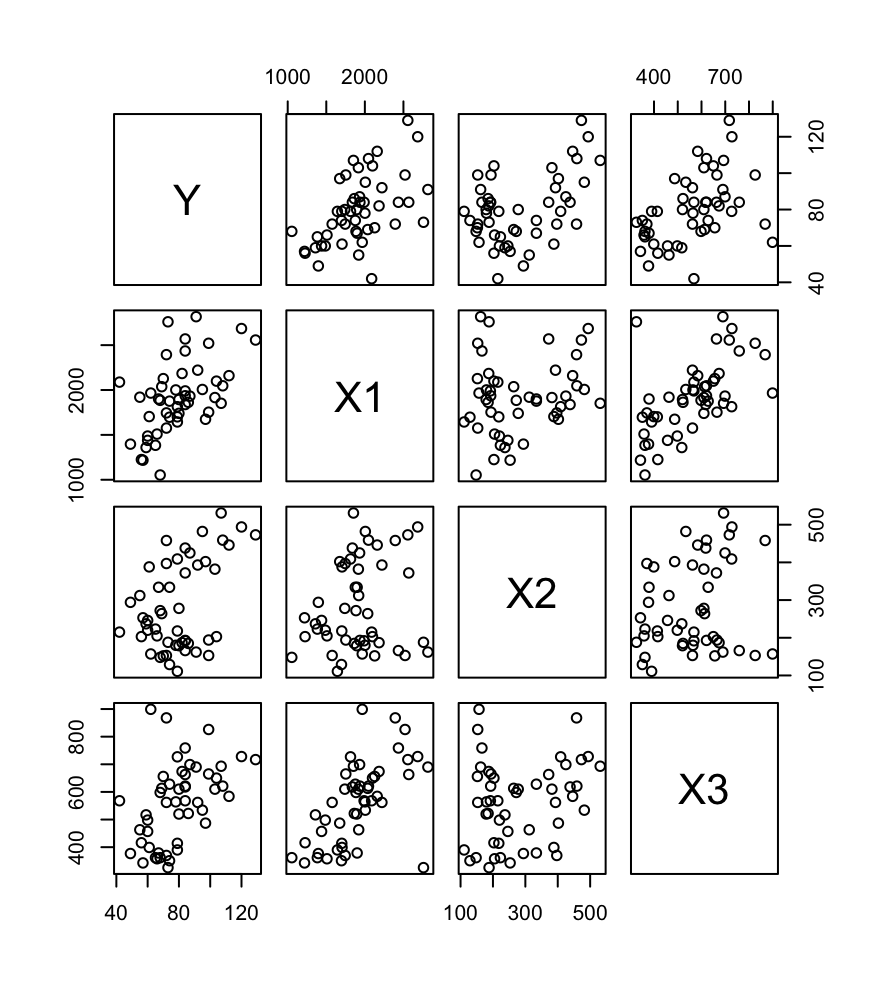
\includegraphics[width=0.5\textwidth]{Rplot01.png}
\end{center}


\item
Please plot the relationship between \emph{Y} and \emph{Region}? On average, which region has the highest per capita expenditure on housing assistance?
		\begin{verbatim}
			#plot(x = expenditure$Region, y = expenditure$Y)
			
			#boxplot(expenditure$Region, expenditure$Y)
			
			
			#factor variables are always categorical variables
			#str(expenditure)
			
			# indexing it like: df[,'x'] <-factor(df)
			# better solution 
			#labels: Northeast = 1,North Central = 2, South = 3, West = 4 
			
			str(expenditure)
			expenditure$Region = factor(expenditure$Region,
			levels = c(1, 2, 3, 4),
			labels = c("Northeast", "North Central", "South", "West"))
			boxplot(formula = expenditure$Y ~ expenditure$Region)
			
			#answer: On average the West region has the highest per capita expenditure on housing assistance 
			
		\end{verbatim}
		
		
		\begin{center}
			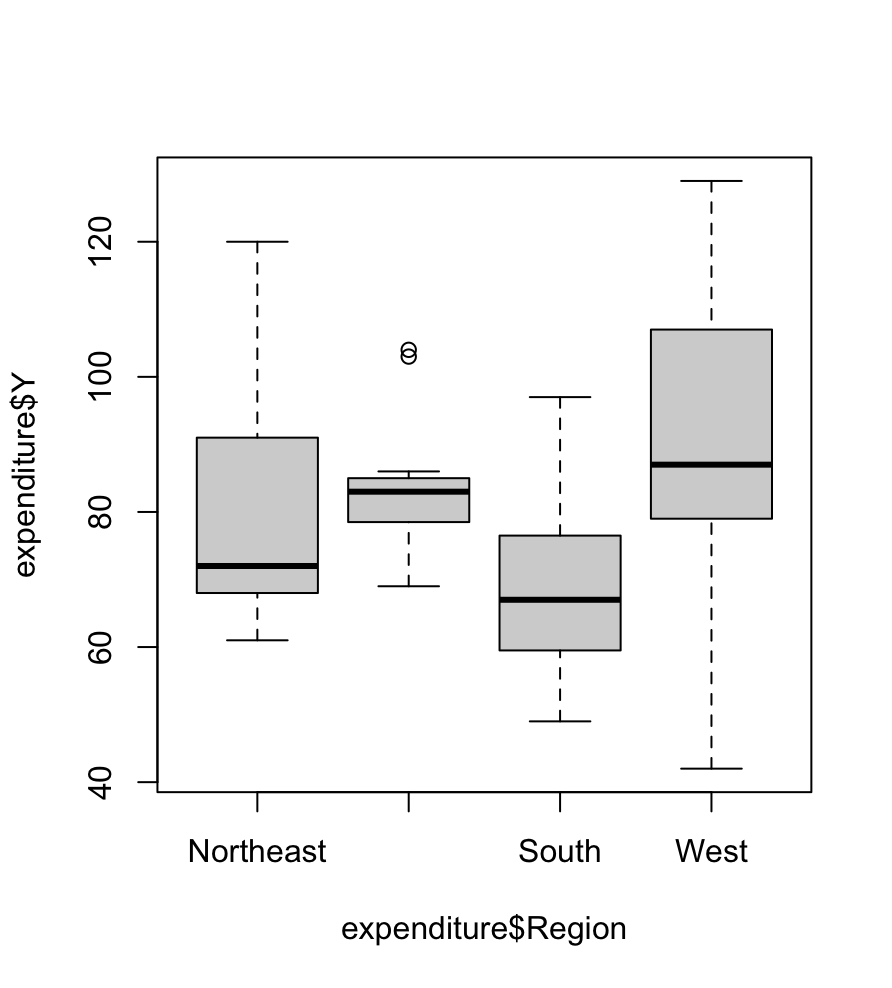
\includegraphics[width=0.5\textwidth]{boxplot1.png}
		\end{center}
		


\vspace{.5cm}
\item
Please plot the relationship between \emph{Y} and \emph{X1}? Describe this graph and the relationship. Reproduce the above graph including one more variable \emph{Region} and display different regions with different types of symbols and colors.

		\begin{verbatim}
			plot(x = expenditure$X1, y = expenditure$Y) 
			
			# answer: There appears to be a positive/moderate assocation between X1 and Y. 
			
			# step 4: reproduce the above graph including one more variable Region and displaydifferent regions with different types of symbols and colors.
			lapply(c("paletteer"),  pkgTest)
			
			colors <- paletteer_c("viridis::inferno", n=4)
			shapes <- c(17, 18, 19, 20)
			
			plot(x = expenditure$X1, 
			y = expenditure$Y,
			col = colors[expenditure$Region],
			pch = shapes[expenditure$Region], 
			cex = 1,
			main = "Spending on housing against per capita income
			(by region)",
			xlab = "per capita income", 
			ylab = "per capita expenditure on housing/shelters")
		\end{verbatim}
\end{itemize}

\begin{center}
	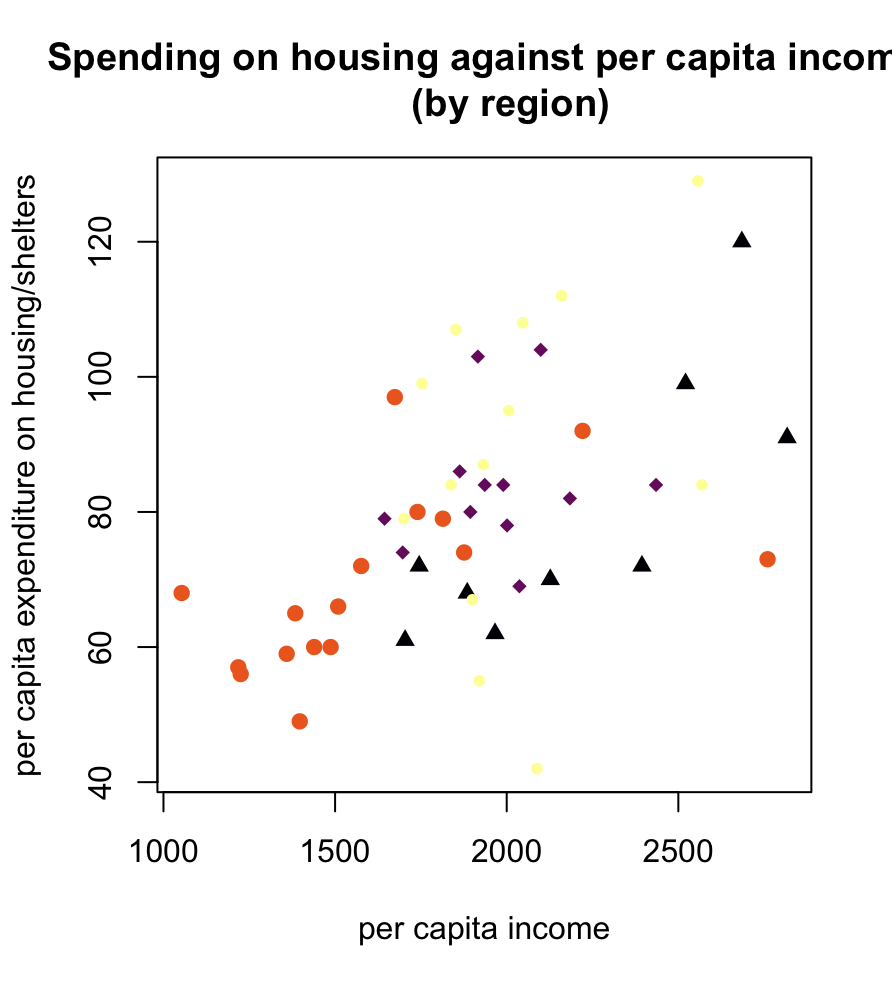
\includegraphics[width=0.5\textwidth]{Rplot.png}
\end{center}


\end{document}
